Chapter covers application and implementation of EKF (Extended Kalman Filter) for estimation of 3D position in space and writing a simulation to validate the filter implementation.

\subsection{EKF}

Due to sensor measurement noise state estimator is necessary. Thus Kalman filter will be implemented and deployed to track agents position assuming noisy observations of distance. Before going into details it's important to think about state evolution and observation models because Kalman filter assumes both to be linear. During project constant velocity model will be used, described by:
$$
    \left[\begin{array}{c}
            x_{k+1}       \\
            y_{k+1}       \\
            z_{k+1}       \\
            \dot{x}_{k+1} \\
            \dot{y}_{k+1} \\
            \dot{z}_{k+1}
        \end{array}\right]=\left[\begin{array}{cccccc}
            1 & 0 & 0 & \Delta t & 0        & 0        \\
            0 & 1 & 0 & 0        & \Delta t & 0        \\
            0 & 0 & 1 & 0        & 0        & \Delta t \\
            0 & 0 & 0 & 1        & 0        & 0        \\
            0 & 0 & 0 & 0        & 1        & 0        \\
            0 & 0 & 0 & 0        & 0        & 1
        \end{array}\right]\left[\begin{array}{c}
            x_{k}       \\
            y_{k}       \\
            z_{k}       \\
            \dot{x}_{k} \\
            \dot{y}_{k} \\
            \dot{z}_{k}
        \end{array}\right]
$$
or
$$
    \boldsymbol{x}_{k+1} = \boldsymbol{F} \boldsymbol{x}_k
$$
which is linear by itself. If it were a system like drone model would be non-linear, more complex and include actuation signal in state transition. Yet the project is aiming at investigating plausibility of localization with UWB antennas rather and experiment will be done by carrying agent device while walking. This cannot be modeled and can be treated as  a black box constant velocity model.
% https://arxiv.org/pdf/2005.00844.pdf (Derivation of a Constant Velocity Motion Model for Visual Tracking) Could be useful ?

However, Euclidean distance measurement model (from beacon to agent) has non-linearity due to the \emph{norm}:
$$
    \Vert\boldsymbol{x}-\boldsymbol{b}\Vert_2 = \sqrt{{\left(\mathrm{b_x}-x\right)}^2+{\left(\mathrm{b_y}-y\right)}^2+{\left(\mathrm{b_z}-z\right)}^2}
$$
where $\boldsymbol{x} = (x,y,z)$ is vector representing agents position and $\boldsymbol{b} = (b_x,b_y,b_z)$ is position of one visible (in radio communication sense) beacon in space. This is where EKF comes into play, the method proposes to use linearized version of non-linear function by taking it's Jacobian and assuming that linearized model representation around a small deviation neighborhood holds true and usa that in place of the measurement matrix $\boldsymbol{H}$. This will be described later but, in short, one can take partial derivatives of the function with respect to each agent's position dimension and evaluate them at current state estimate. For instance:
$$
    \frac{\partial h(x)}{\partial x} = \frac{x-\mathrm{b_x}}{\sqrt{{\left(\mathrm{b_x}-x\right)}^2+{\left(\mathrm{b_y}-y\right)}^2+{\left(\mathrm{b_z}-z\right)}^2}}
$$

General discrete time EKF is defined as described in the following paragraphs, based on \cite{probrobotics} and \cite{welch1995introduction}. Starting with notation: $\hat{\mathbf{x}}_{k \mid k-1}$ represents the  estimate of $\mathbf{x}$ at time instance $k$ given observations up to and including at time $k-1$. \smallskip
% TODO: define all variables in EKF ?

\textbf{Prediction step} \smallskip
$$\hat{\boldsymbol{x}}_{k \mid k-1}=f\left(\hat{\boldsymbol{x}}_{k-1 \mid k-1}, \boldsymbol{u}_k\right)$$
$$\boldsymbol{P}_{k \mid k-1}=\boldsymbol{F}_k \boldsymbol{P}_{k-1 \mid k-1} \boldsymbol{F}_k^T+\boldsymbol{Q}_k$$

\textbf{Update step} \smallskip
$$\tilde{\boldsymbol{y}}_k=\boldsymbol{z}_k-h\left(\hat{\boldsymbol{x}}_{k \mid k-1}\right)$$
$$\boldsymbol{S}_k=\boldsymbol{H}_k \boldsymbol{P}_{k \mid k-1} \boldsymbol{H}_k^T+\boldsymbol{R}_k$$
$$\boldsymbol{K}_k=\boldsymbol{P}_{k \mid k-1} \boldsymbol{H}_k^T \boldsymbol{S}_k^{-1}$$
$$\hat{\boldsymbol{x}}_{k \mid k}=\hat{\boldsymbol{x}}_{k \mid k-1}+\boldsymbol{K}_k \tilde{\boldsymbol{y}}_k$$
$$\boldsymbol{P}_{k \mid k}=\left(\boldsymbol{I}-\boldsymbol{K}_k \boldsymbol{H}_k\right) \boldsymbol{P}_{k \mid k-1}$$
where state transition and measurement matrices are partial derivatives (\emph{Jacobians}) of state evolution and observation model functions. In constant velocity case $\boldsymbol{f}(\boldsymbol{x})$ is already linear so that part can be discarded.
$$
    \begin{aligned}
        \boldsymbol{F}_k & =\left.\frac{\partial f}{\partial \boldsymbol{x}}\right|_{\hat{\boldsymbol{x}}_{k-1 \mid k-1}, \boldsymbol{u}_k} \\
        \boldsymbol{H}_k & =\left.\frac{\partial h}{\partial \boldsymbol{x}}\right|_{\hat{\boldsymbol{x}}_{k \mid k-1}}
    \end{aligned}
$$

Distance measurement Jacobian can be computed in code by:

\begin{minipage}{\linewidth}
    \begin{python}
    def getH(x_op, beacons):
        H = np.zeros((len(beacons), len(x_op)))
        for i, b in enumerate(beacons):
        H[i][:3] = ((x_op[:3] - b.get_pos()) \
            / np.linalg.norm(x_op[:3] - b.get_pos())).T
        return H
    \end{python}
\end{minipage}
% doesn't stay formatted as i wish if i wrap it :'( despair
% \begin{figure}
%     \caption{Distance Jacobian $\boldsymbol{H} computation.$}
%     \label{code:distJ}
% \end{figure}
function takes in agent position at time $k-1$, beacon list and return partial derivatives of state variables with respect to each of the beacons. It's assumed that beacon number is fixed to 4.

\subsection{Simulation}

Figure \ref{fig:sim} shows a trail run in simulation. Please note that system state is includes the third dimension however for plotting purpose only first two components are shown. The setup is running EKF described in previous section on noisy measurement. Noise is provided by adding a random sample from Gaussian distribution to each distance measurement at every timestamp. Big $X$ is marking the start of a trajectory, $GT$ line is ground truth trajectory generated by applying state transition matrix at each instant of time (moving at arbitrary speeds to cover a rectangle), blue path is the predicted one and lastly the numbered dots represent beacons arbitrarily placed in space.
\begin{figure}[H]
    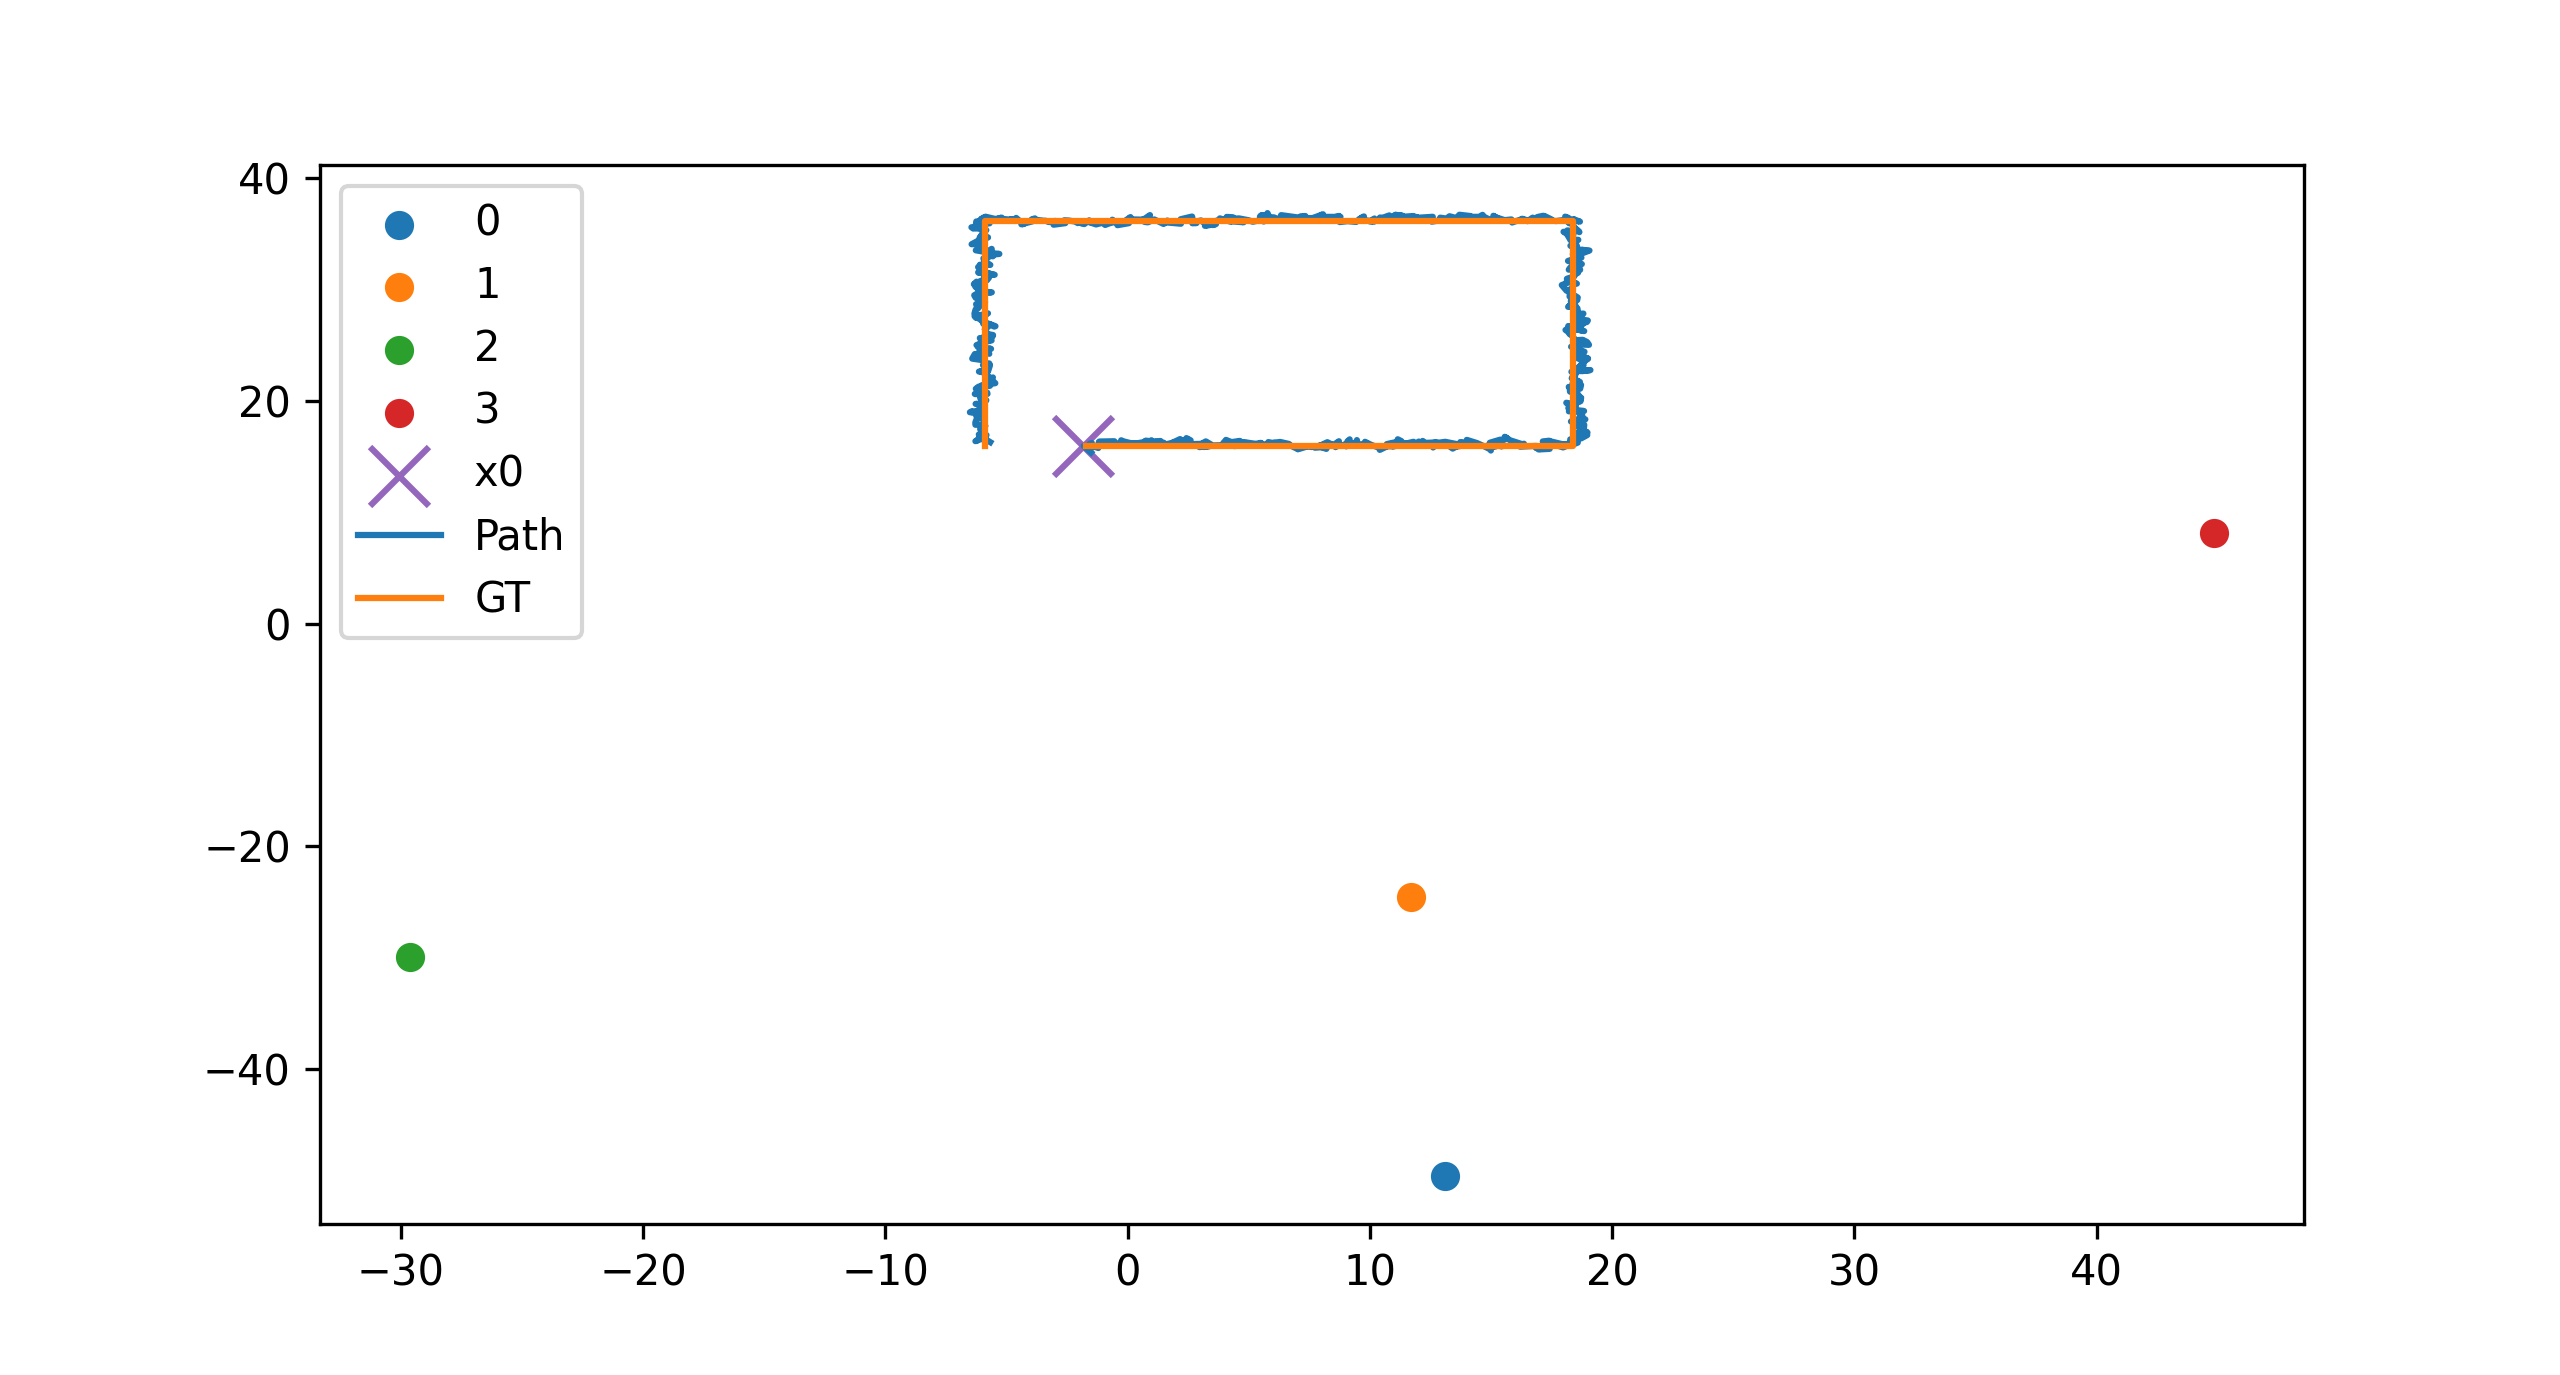
\includegraphics[width=\linewidth]{figures/sim.png}
    \caption{Simulation}
    \label{fig:sim}
\end{figure}